\documentclass{esannV2}
\usepackage{subfig}
\usepackage{color}
\usepackage{url}
 
% My packages
\usepackage{ctable} % for \specialrule command
%\usepackage{tikz}
%\usepackage{pgfplots}
%\usepackage{filecontents}
%\usepackage{amsfonts}
%\usepackage{booktabs}
%\usepackage{amsthm}
\usepackage{amssymb,amsmath,array}
\usepackage[utf8]{inputenc}
%\usepackage{color}
%\usepackage{algorithm}
%\usepackage{algorithmic}
%\usepackage{multirow}
%\usepackage{array}
%\usepackage{subfig}
%\usepackage{caption}
%\usepackage{graphicx}
%\usepackage{hyperref}
%\usepackage{algorithmicx}
%\usepackage{float}
%\usepackage{soul}
%\usepackage{amsfonts}
%\usepackage{subfigure}
\usepackage{amsbsy}
%\usepackage{setspace}
%\usepackage{hyperref}
%\usepackage[bookmarks=false]{hyperref}
%\usepackage{babel,blindtext}
\usepackage{color}

% My commands
\newcommand{\Real}{\mathbb{R}}
\newcommand{\Natu}{\mathbb{N}}
\newcommand{\dd}{{\bf d}}
\newcommand{\xx}{{\bf x}}
\newcommand{\yy}{{\bf y}}
\newcommand{\zz}{{\bf z}}
\newcommand{\ff}{{\bf f}}
\newcommand{\ww}{{\bf w}}
\newcommand{\vv}{{\bf v}}
\newcommand{\AAA}{{\bf A}}
\newcommand{\CC}{{\bf C}}
\newcommand{\DD}{{\bf D}}
\newcommand{\EE}{{\bf E}}
\newcommand{\GG}{{\bf G}}
\newcommand{\KK}{{\bf K}}
\newcommand{\YY}{{\bf Y}}
\newcommand{\MM}{{\bf M}}
\newcommand{\HH}{{\bf H}}
\newcommand{\II}{{\bf I}}
\newcommand{\XX}{{\bf X}}
%\newcommand{\NN}{{\bf N}}
\newcommand{\cU}{{\cal U}}
\newcommand{\cI}{{\cal I}}
\newcommand{\cR}{{\cal R}}
\newcommand{\cN}{{\cal N}}
\newcommand{\cQ}{{\mathcal Q}}
\newcommand{\1}{{\bf 1}}
\newcommand{\Exp}{\mathbb{E}}
\newcommand{\labelfun}{L}
\newcommand{\node}{v}
\newcommand{\cK}{{\cal K}}
%\newtheorem{lemma}{Lemma}
%\newtheorem{theorem}{Theorem}
%\newtheorem{corollary}{Corollary}
%\newtheorem{proposition}{Proposition}
%\newtheorem{definition}{Definition}
%\newtheorem{remark}{Remark}
\newcommand{\cC}{{\cal C}}
\newcommand{\R}{{\mathbb R}}
\newcommand{\N}{{\mathbb N}}
\newcommand{\ggamma}{\pmb{\gamma}}
\newcommand{\aalpha}{\pmb{\alpha}}
\newcommand{\bbeta}{\pmb{\beta}}
\newcommand{\eeta}{\pmb{\eta}}
\newcommand{\ssigma}{\pmb{\sigma}}
\newcommand{\llambda}{\pmb{\lambda}}
\newcommand{\mmu}{\pmb{\mu}}
\newcommand{\pphi}{\pmb{\phi}}

\newcommand{\res}[2]{$#1_{\pm#2}$}

\newcommand{\kval}{$K_{\textsc{val}}$}
\newcommand{\ksum}{$K_{\textsc{sum}}$}
\newcommand{\kmkl}{$K_{\textsc{mkl}}$}
\newcommand{\ksmkl}{$K_{\textsc{mkl}}^{sub}$}
\newcommand{\kssum}{$K_{\textsc{sum}}^{sub}$}
\newcommand{\ksw}{$K_{\textsc{w}}^{sub}$}
\newcommand{\tb}[1]{\boldsymbol{#1}}


\renewcommand{\baselinestretch}{.96}

%***********************************************************************
% !!!! IMPORTANT NOTICE ON TEXT MARGINS !!!!!
%***********************************************************************
%
% Please avoid using DVI2PDF or PS2PDF converters: some undesired
% shifting/scaling may occur when using these programs
% It is strongly recommended to use the DVIPS converters, and to submit
% PS file. You may submit a PDF file if and only if you use ADOBE ACROBAT
% to convert your PS file to PDF.
%
% Check that you have set the paper size to A4 (and NOT to letter) in your
% dvi2ps converter, in Adobe Acrobat if you use it, and in any printer driver
% that you could use.  You also have to disable the 'scale to fit paper' option
% of your printer driver.
%
% In any case, please check carefully that the final size of the top and
% bottom margins is 5.2 cm and of the left and right margins is 4.4 cm.
% It is your responsibility to verify this important requirement.  If these margin requirements and not fulfilled at the end of your file generation process, please use the following commands to correct them.  Otherwise, please do not modify these commands.
%
\voffset 0 cm \hoffset 0 cm \addtolength{\textwidth}{0cm}
\addtolength{\textheight}{0cm}\addtolength{\leftmargin}{0cm}

%***********************************************************************
% !!!! USE OF THE esannV2 LaTeX STYLE FILE !!!!!
%***********************************************************************
%
% Some commands are inserted in the following .tex example file.  Therefore to
% set up your ESANN submission, please use this file and modify it to insert
% your text, rather than staring from a blank .tex file.  In this way, you will
% have the commands inserted in the right place.



\begin{document}
%style file for ESANN manuscripts
%primo tentativo
\title{Fast Hyper-Parameter Selection for Graph Kernels via Subsampling and\\Multiple Kernel Learning}

%***********************************************************************
% AUTHORS INFORMATION AREA
%***********************************************************************
%\author{First author$^1$ and Second author$^2$
\author{Michele Domini$^1$, Nicol\`o Navarin$^2$, Ivano Lauriola$^2$, Fabio Aiolli$^2$ and Fabrizio Costa$^3$
%
% Optional short acknowledgment: remove next line if non-needed
%\thanks{This is an optional funding source acknowledgement.}
%
% DO NOT MODIFY THE FOLLOWING '\vspace' ARGUMENT
\vspace{.3cm}\\
%
% Addresses and institutions (remove "1- " in case of a single institution)
1- Computational Statistics and Machine Learning (CSML) \\
Istituto Italiano di Tecnologia, Via Morego 30, Genova, Italy
\vspace{.1cm}\\
2- Department of Mathematics, University of Padova\\
via Trieste 63, Padova, Italy
\vspace{.1cm}\\
3- ... \\
...
}

%commento sta roba
%1- School of First Author - Dept of First Author \\
%Address of First Author's school - Country of First Author's
%school
%
% Remove the next three lines in case of a single institution
%\vspace{.1cm}\\
%2- School of Second Author - Dept of Second Author \\
%Address of Second Author's school - Country of Second Author's school\\
%}
%***********************************************************************
% END OF AUTHORS INFORMATION AREA
%***********************************************************************

\maketitle

%\renewcommand{\baselinestretch}{.95}

\begin{abstract}
Kernel for structures are generally characterized by a number of hyper-parameter which need to be tuned. Moreover, different types of kernels can be used and the best choice usually depends on data. The hyper-parameter setting is a time-consuming step. One option proposed to overcome this problem is to use the Multiple Kernel Learning approach and generate a kernel which is a combination of different types of kernels and different hyper-parameters settings. However, this solution still requires the computation of many large kernel matrices. In this paper we propose a subsampling method to efficiently select a small number of kernels which need to be actually computed. Finally, we give empirical evidence that the method proposed is far more efficient than the other approaches while maintaining similar results in terms of AUC.
\end{abstract}


\section{Introduction}
In different real-world domains, it may be easy to encode examples in a structured form. For example, in chemoinformatics there is a well known graph representation of the secondary structures of chemical compounds. Moreover, images can easily be represented as graph after segmentation, where adjacent objects (or regions) are linked.
In these cases, deriving a vectorial representation for the data may be a time-consuming task, where information from  domain experts is needed, and information loss is, in general, unavoidable.
Another option is to deal directly with examples represented in a structured form.
In this case, specific machine learning techniques have to be adopted.
Kernel methods are one option, where it suffices to adopt a kernel function defined for data type under consideration. Then, standard (kernelized) learning algorithms (e.g. SVM) can be adopted.

With kernel methods, a user has usually to deal with several of hyper-parameters to fix manually. The optimization of these hyper-parameters can strongly affect the predictive performance of the method.
Usually, these parameters are: (i) the choice of the kernel to adopt; (ii) the hyper-parameters of the selected kernel; (iii) the hyper-parameters of the learning algorithm.
A commonly adopted and simple approach to hyper-parameters optimization is to fix a-priori some possible values for each parameter (the combinations of these parameters are referred to as \textit{parameters grid}).
Then, the learning algorithm is trained for each possible parameters combination, and its performances are evaluated. This approach is commonly referred to as grid-search.

With this approach, a learning procedure has to be performed for each hyper-parameter combination, possibly making it very time consuming.
A possible alleviation to this problem has been proposed in~\cite{Massimo2016}, where Multiple Kernel Learning (MKL) has been used for combining different kernel matrices in a single learning procedure, instead of selecting the best parameters configuration.
However, in the case of kernel algorithms, a different kernel matrix has to be computed for each kernel and for each of its hyper-parameters values in the grid. This step can also be time consuming, especially when dealing with data in a structured form.

In this paper, we propose a new approach to parameter selection that, based on sub-sampling and MKL, is able to speedup the parameter selection phase by orders of magnitude on real-world datasets.

%\section{Kernel for structures and Multiple Kernel Learning}
\section{Background}
A kernel method is composed by the following two modules.
A learning algorithm, that expresses the solution only via dot products between training examples.
A kernel function ${k}: \mathcal{X} \times \mathcal{X} \rightarrow \mathbb{R}$ that is a symmetric positive semi-definite function that corresponds to a dot product in a Reproducing Kernel Hilbert Space (RKHS), i.e. there exists a $\phi: \mathcal{X} \rightarrow \mathcal{K} \subseteq \mathbb{R}^D$, where $\mathcal{X}$ is the input space and $\mathcal{K}$ is an Hilbert space (commonly referred to as \textit{feature space}), such that $k(x_i,x_j) = \langle \phi(x_i),\phi(x_j) \rangle$ with $x_i,x_j \in \mathcal{X}$. %~\cite{559923}.
%\textcolor{red}{TODO definire kernel matrix}
A kernel (or \textit{Gram}) matrix for a set of examples $Tr=\{x_1, \ldots, x_l\}$ is an $l \times l$ matrix $G$ with entries $\{G\}_{ij}=k(x_i,x_j)$.
When dealing with structured data, the choice of the kernel to adopt is a key step. Depending on the type of data under consideration, different proposals are available in literature, each one with a different trade-off between expressiveness and efficiency.
%(of course, this trade-off depends from the considered task).

In this paper we focus on graphs, i.e. we consider each example to be a different graph.
A graph is a tuple $G=(V_G,E_G,L_G)$, where $V_G=\{v_1,\ldots,v_n\}$ is the set of vertices, $E_G=\{(u,v) | u,v \in V_G\}$ is the set of edges (with $|E_G|=m$), and $L_G: V_G \rightarrow \Sigma$ is a function mapping each vertex to a discrete label in a fixed alphabet $\Sigma$.
%A graph is undirected if $(u,v)\in E_g \Rightarrow (v,u) \in E_G$, otherwise it is directed.
In this setting, there are several graph kernels defined in literature based on random walks~\cite{Kashima03marginalizedkernels,Mahe2004} ($O(n^3)$ computational complexity), shortest paths~\cite{Kriegel05shortestpath} ($O(n^4)$ computational complexity), subgraphs up to a fixed size $h$~\cite{Shervashidze2009} ($O(n^h)$ complexity). The problem with these kernels is the high computational complexity, that makes them inapplicable to several real-world datasets.
Recently, different almost linear time graph kernels have been defined in literature \cite{Heinonen2009,Costa2010,Shervashidze2011,Dasan2012,DaSanMartino2016}, and these are the ones we focus on in this paper.
%In the following we will give some details about the considered alternatives.
Each one of these kernels considers only specific kinds of subgraphs, up to a certain dimension (that, in general, is a kernel parameter).
Note that it is out of the scope of this paper to give an extensive comparison among the various graph kernels. 

The Weisfeiler-Lehman Fast Subtree kernel (WL)~\cite{Shervashidze2011}  counts the number of identical subtree patterns obtained by subtree-walks up to height $h$ (an hyper-parameter) in the two input graphs. The complexity of the kernel is $O(|E|h)$. 
%While being fast to compute, the kernel may lack of expressiveness for some tasks given that the number of non-zero features generated by one graph is at most $|V|h$. 
Note that the subtree-walks extracted by the kernel differ from  subtree structures because a node can appear multiple times in the same subtree-walk.

In~\cite{Costa2010} the Neighborhood Subgraph Pairwise Distance Kernel (NSPDK) is presented. This kernel computes the exact matches between pairs of subgraphs with controlled size and distance (hyper-parameters $r$ and $d$, respectively). 
The kernel has $O(|V| |V_h| |E_h| \log |E_h|)$ time complexity, where $|V_h|$ and $|E_h|$ are the number of nodes and the number of edges of the subgraph obtained by a breadth-fist visit of depth $h$. 
% The complexity of the kernel is $O(|V| |V_h| |E_h| \log |E_h|)$, where $|V_h|$ and $|E_h|$ are the number of nodes and the number of edges of the subgraph obtained by a breadth-fist visit of depth $h$. 
The authors state that, for small values of the subgraph size and distance, the complexity of the kernel becomes in practice linear.

The Ordered Decomposition DAGs Subtree kernel (ODD$_{ST}$)~\cite{Dasan2012,DaSanMartino2016} considers as non-zero features in the RKHS the trees that appear as subtrees of the input graphs.
It exploits the shortest-path (up to length $h$, a hyper-parameter) DAG decompositions starting from each node in the graph to generate DAG structures, and then extracts tree features from them.
Each tree-feature is weighted as $f \cdot \lambda^{dim}$, where $f$ is the frequency of the feature, $dim$ its dimension (the number of vertices in the tree) and $\lambda>0$ a weighting hyper-parameter.
The time complexity of the kernel is, under mild conditions, $O(|V_G| \log |V_G|)$.%, and the number of generated features for a graph is at most $|V_G|\rho^\eta$.

\subsection{Multiple Kernel Learning}
\label{MKL}
MKL \cite{Gonen2011} is one of the most popular paradigms used to learn kernels in real world applications \cite{Bucak2014,Castro2014}. % Zien2007,Wang2015a,Sun
The kernels generated by these techniques are combinations of a prescribed set of basic kernels $\KK_1,...,\KK_R$ with a constraint in the form:
$
	H_R^q = \{ \xx \mapsto \textbf{w} \cdot \pphi_\KK(\xx) : \KK = \sum_{r=1}^R \eta_r \KK_r, \mmu \in \Psi_q, \|\textbf{w}\|_2 \leqslant 1 \}
$
with $\Psi_q = \{ \mmu : \mmu \succcurlyeq 0, \| \mmu \|_q = 1 \}$ and considering the function $\pphi_\KK$ as the feature mapping from the input space to the feature space. The value $q$ being the kind of mean used, is typically fixed to $1$ or $2$.

Using this formulation, we are studying the family of sums of kernels in the feature space. It is well know that the sum of two kernels can be seen as the concatenation of the features contained in both the RKHS \cite{Shawe-Taylor2004}. Extending the same idea, the weighted sum of a list of basic kernels can be seen as a weighted concatenation of all the features contained in all the RKHS (where the weights are the square roots of the learned weights $\eta_k$).

 %structured sparsity regularizers \cite{Micchelli2010,Micchelli2013}.
%The problem of searching for a combinations of basic kernels can be rephrased as a regularization problem in which the prediction function is the sum of functions $f_r$ in the RKHS of kernel $\KK_r$ and the regularization term is the combination of the norms of the $f_r$ in the associated RKHS \cite{Micchelli2005a}. %,Micchelli2007
%For example if $q=1$ this is a parametric version of the group Lasso \cite{Meier2009}, see e.g. \cite{Maurer2012}.

These algorithms are supported by several theoretical results that bound the \emph{estimation error} (i.e. the difference between the true error and the empirical margin error). These bounds exploit the \emph{Rademacher complexity} applied to the combination of kernels \cite{Maurer2012,Cortes2009c}%,Hussain2011,Hussain2011a}. %,Kakade2009,Micchelli2005,Kloft2012,Srebro2006,

Existing MKL approaches can be divided in two main categories. In the first category, \emph{Fixed or Heuristic}, some fixed rule is applied to obtain the combination. They usually get results scalable with respect to the number of kernels combined but their effectiveness critically depends on the domain at hand. %They use a parameterized combination function and find the parameters of this function generally by looking at some measure obtained from each kernel separately,  often giving a suboptimal solution (since no information sharing among the kernels is exploited).

On the other hand, the \emph{Optimization based} approaches learn the combination parameters by solving a single optimization problem directly integrated in the learning machine %(e.g. structural risk based target function)
or formulated as a different model (e.g. alignment, or other kernel similarity maximization) \cite{Rakotomamonjy2008,Varma2009}. %,Kloft2011,SorenSonnenburg2006,Vishwanathan2010,Xu2010,Bach2004

%*** good refs. [F. R. Bach, R. Jenatton, J. Mairal, and G. Obozinski. Optimization with sparsity-inducing penalties. Foundations and Trends in Machine Learning, 4:1?106, 2011.] \cite{Bach2012} ***

\subsubsection{EasyMKL}
\label{EasyMKL}
EasyMKL \cite{Aiolli2015} is a recent MKL algorithm able to combine sets of basic kernels by solving a simple quadratic optimization problem. Besides its proved empirical effectiveness, a clear advantage of EasyMKL compared to other MKL methods is its high scalability with respect to the number of kernels to be combined. Specifically, its computational complexity is constant in memory and linear in time.
EasyMKL finds the coefficients $\boldsymbol{\eta}$ that maximize the margin on the training set, where the margin is computed as the distance between the convex hulls of positive and negative examples. In particular, the general problem EasyMKL tries to optimize is the following:
\vspace{-0.4cm}
\begin{equation}
\label{eq:easymklotig}
\max_{\boldsymbol{\eta}:||\boldsymbol{\eta}||_2=1} \min_{\boldsymbol{\gamma} \in \Gamma} \mbox { }  \boldsymbol{\gamma}^{\top} \YY ( \sum_{r=0}^R \eta_r \KK_r) \YY \boldsymbol{\gamma} + \Lambda ||\boldsymbol{\gamma}||^2,
\end{equation}
%\vspace{-0.1cm}
where $\YY$ is a diagonal matrix with training labels on the diagonal, and $\Lambda$ is a regularization hyper-parameter. The domain $\Gamma$ represents two probability distributions over the set of positive and negative examples of the training set, that is $\Gamma = \{\boldsymbol{\gamma} \in \Real_+^{\ell} \hspace{0.2cm} |  \sum_{y_i = +1} \boldsymbol{\gamma}_i = 1 , \sum_{y_i = -1} \boldsymbol{\gamma}_i = 1\}.
$
Note that any element $\boldsymbol{\gamma} \in \Gamma$ corresponds to a pair of points, the first in the convex hull of positive training examples and the second in the convex hull of negative training examples.
At the solution, the first term of the objective function represents the obtained margin, that is the (squared) distance between a point in the convex hull of positive examples and a point in the convex hull of negative examples, in the compounded feature space.
%The objective function in Eq. \ref{eq:easymklotig} can be interpreted as the dual problem of a regularized empirical objective function using the kernel $\sum_{r=1}^R \eta_r \KK_r$.
Eq. \ref{eq:easymklotig} is a minimax problem that can be reduced  to a simple quadratic problem with a technical derivation described  in \cite{Aiolli2015}. %The solution of the quadratic problem is an optimal $\ggamma^*$ for the original min-max formulation. Due to the particular structure of EasyMKL, it is sufficient to provide the average kernel of all the basic kernels ($\KK^A = \frac{1}{R} \sum_{r=1}^R \frac{\KK_r}{Tr(\KK_r)}$). From $\ggamma^*$, it is easy to obtain the optimal weights for the single basic kernels $\KK_r$ by using the following formula
%\begin{equation}
%\label{eq:easyeta}
%	\eta_r = \gamma^{*T} \YY \,\, (\KK_r/Tr(\KK_r)) \,\, \YY \gamma^*, \,\,\,\, \forall r=1,\dots,R.
%\end{equation}
In the following sections, we will refer to this method as EasyMKL\footnote{EasyMKL implementation: github.com/jmikko/EasyMKL}.
%and we have to provide it only $\KK^A$, the dataset $\XX$ and $\yy$ to evaluate equation \ref{eq:easyeta}, and the EasyMKL regularization hyper-parameter $\Lambda$.


\section{Proposed framework}
Often, to work well MKL algorithms require an high number of kernels, and when we use structured data as input, such as graphs, the computational effort to calculate each of them can be high. Moreover each kernel requires an amount of memory that depends on the number of samples, making the MKL approach unpractical when the number of samples and the number of kernels are huge.
In order to avoid these problems, we propose a method to reduce the number of kernels to compute on the complete dataset, based on the robustness of the combination vector $\boldsymbol{\eta}$ when considering just a subset of the available data.\\
In particular if $\boldsymbol{\eta}$, the combination vector learned using the whole set of data and all kernel functions, is similar to the weights vector $\hat{\boldsymbol{\eta}}$ learned using the same kernels calculated on a subset of data, we can compute just $\hat{\boldsymbol{\eta}}$ .
%In this way we can learn quickly the kernels combination, but we have to calculate all kernels anyway.
Moreover, we can use the values in $\hat{\boldsymbol{\eta}}$ to perform a ranking over kernels, removing those below a (user-specified) threshold.
Then we compute the kernel matrix, on all the available data, for just the top kernels, and fit a model combining them.

%In summary, in the first phase we choose the top kernels using a subset of the available data. In the second phase, we calculate the top kernel matrices using the whole set of data, and then we use them in combination.


\section{Experimental Assessment}
We conducted our experiments on several real-world binary datasets, that are MUTAG, CPDB, GDD, AIDS, NCI1, NCI109, CAS (see \cite{DaSanMartino2016} for a more detailed description).
%AIDS~\cite{Weislow1989a}, CAS\footnote{http://cheminformatics.org/datasets/bursi/},
%CPDB~\cite{Helma2004a}, NCI1~\cite{Wale2006} and GDD~\cite{dobson2003}.
%The first four datasets contain chemical particles encoded in graph form, while the latter encodes proteins.
{\color{red} The AIDS dataset contains chemical compounds (encoded in graph form), labeled according to
their antiviral activity; CAS and CPDB store compounds labeled according to their mutagenicity; NCI1 and NCI109 consist of chemical compounds screened for activity against non-small lung cancer cells; GDD is composed of X-ray crystal structures of proteins; MUTAG contains %MUTAG serve per far vedere che funziona bene anche su dataset piccolissimi
[...].
All the nodes are labeled and there are no self loops.}

The kernels used in our experiments are: all NSPDK combinations with $h \in \{0,1\dots9\}$ and $d \in \{0,1\dots9\}$, all ODDST combinations with $h \in \{0,1\dots9\}$ and $\lambda \in \{0.5, 0.7,0.8\dots1.2,1.4,1.6,1.8\}$, all WL with $h \in \{0,1\dots9\}$.
In all models, we considered kernels calculated in less that 1 hour, rejecting others.
The baselines used to compare our method consist on a SVM with kernels (a)\kval: the kernel is the one which has the best validation score, (b)\ksum: the kernel is the average of all base kernels, (c)\kmkl: the kernel is a combination of all base kernels using EasyMKL.
For each baseline, the computation of all kernels is required.
The hyperparameters are chosen using a nested 10-fold CV procedure, and they are $C\in\{2^i, i:-3\dots6\}$, and $\Lambda\in\{0,0.1\dots1\}$ for \kmkl.


Firstly, we performed some experiments to check how many samples are required to make $\boldsymbol{\eta}$ and $\hat{\boldsymbol{\eta}}$ similar.
In our context two weights vectors are similar if they provide the same top kernels. By the way the metric used for comparison is the jaccard similarity score. \figurename\ \ref{fig:jaccard} shows the Jaccard score between the indices of top kernels selected using $\boldsymbol{\eta}$ and $\hat{\boldsymbol{\eta}}$ with different threshold and different subsampling dimension.
According to other preliminary results, we fix the dimension of subset used in the first step to learn $\hat{\boldsymbol{\eta}}$ as 10\% and the number of top kernels as 10\%. Except for MUTAG, where we use 20\% of training data.

\begin{figure}[!htb]
\centering
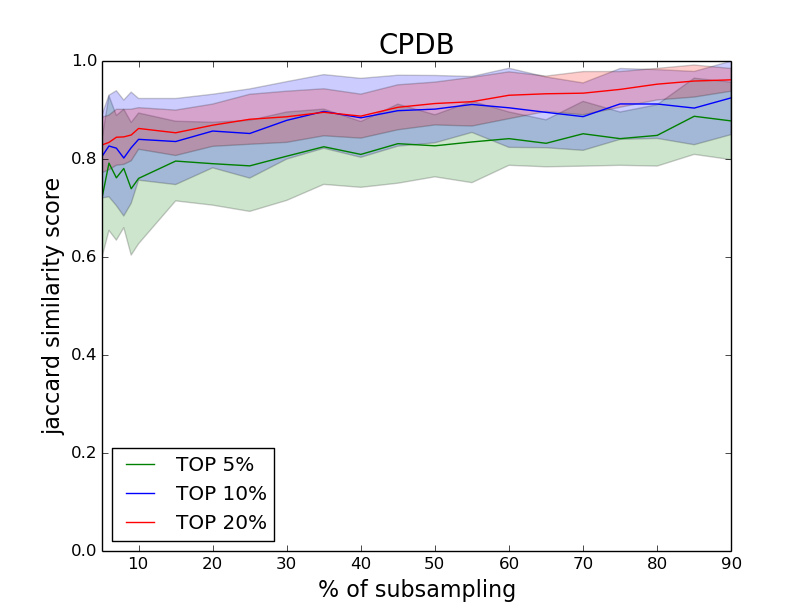
\includegraphics[width=0.42\textwidth]{img/CPDB_jaccard.png}
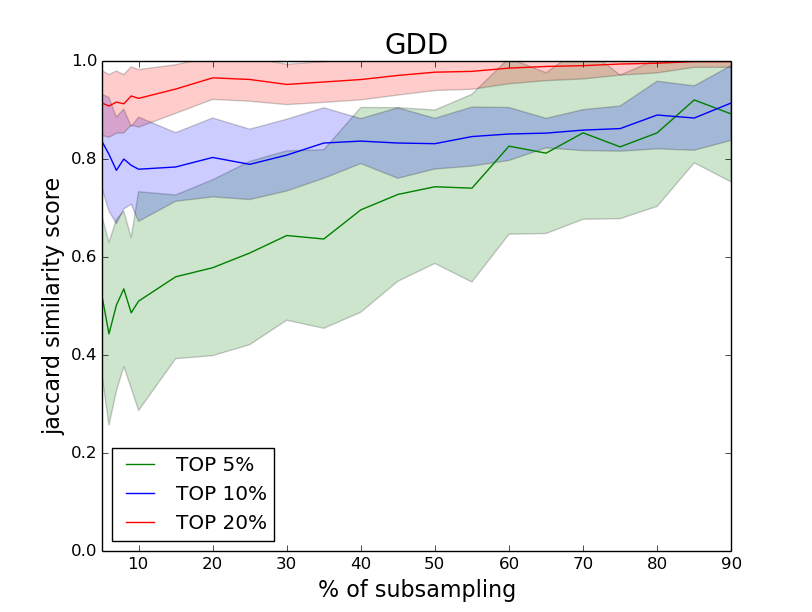
\includegraphics[width=0.42\textwidth]{img/GDD_jaccard.png}
\caption{Average jaccard values and standard deviation in 50 runs between the indices of top kernels using a subset of training data and using the whole set.}
\label{fig:jaccard}
\end{figure}

To learn $\hat{\boldsymbol{\eta}}$ we chose a random subsampling of training data and perform a 10-fold cross validation using EasyMKL to combine kernels and SVM as base learner. Then we fit the model with the best combination and select the top kernels.
In the second step we calculate the top kernel matrices using the whole training data and combine it to get the kernel. We propose 3 different methods to perform this combination:
(1)\ksmkl: using the EasyMKL algorithm, (2)\kssum: calculating the average of kernels, (3)\ksw: using the same weights (rescaled) from the first learning step.
In all of these methods we use a SVM as base learner. The hyperparameters sets are the same used in baselines.\\
\tablename\ \ref{tab:res} shows the AUC score, standard deviation and computation time used to make kernels and models for all problems.


\begin{table}[]
\centering
\resizebox{\textwidth}{!}{
\begin{tabular}{l|c|ccc|ccc}
\hline\hline
dataset & \# train &\kval &\kmkl &\ksum & \ksmkl & \kssum & \ksw \\
\hline
MUTAG   & 188 & \res{0.9023}{0.075} & \res{0.9310}{0.061} & \res{0.9309}{0.060} & \res{0.9292}{0.054} & \res{0.9292}{0.054} & \res{\tb{0.9331}}{0.053}    \\
&			  & 18m					& 40m				& 8m		& 3m		&4m		&4m\\\hline
CPDB    & 684 &$0.8753_{\pm0.029}$ & $0.8814_{\pm0.027}$ & $0.8809_{\pm0.029}$ & $0.8768_{\pm0.023}$ & $\tb{0.8850}_{\pm0.027}$ & $0.8751_{\pm0.023}$ \\
&			  & 1h 16m				& 8h 33m		& 20m	& 1h 37m		& 5m		&5m\\\hline
GDD     & 1178 & \res{0.8647}{0.045} & \res{\tb{0.8719}}{0.039} & \res{0.8675}{0.039} & \res{0.8690}{0.041} & \res{0.8713}{0.043} & \res{0.8011}{0.036}    \\
&			& $>$100h	& $>$100h	& $>$100h	&3h		& 4h 15m		& 4h 15m\\\hline
AIDS    & 1503 & \res{0.7797}{0.083} & \res{0.7775}{0.080} & \res{0.7712}{0.083} & \res{\tb{0.7845}}{0.077} & \res{0.7690}{0.074} & \res{0.7673}{0.073}    \\
&		& 6h 39m		& 50h	& 2h 44m		& 11h 10m	& 1h 4m	& 1h 4m\\\hline
NCI1    & 4110 & \res{0.8839}{0.043} & - & \res{\tb{0.8851}}{0.041} & \res{0.8818}{0.043} & \res{0.8772}{0.047} & \res{0.8811}{0.044}    \\
&	&	39h	&-	& 7h 24m		& 98h	& 2h 1m	& 2h 1m\\\hline
NCI109 & 4127 & \res{\tb{0.8728}}{0.025} & - & \res{0.8713}{0.025} & \res{0.8670}{0.024}  & \res{0.8713}{0.025} & \res{0.8680}{0.022}  \\
&	&	44h	&-	& 7h 36m		& 99h	& 1h 47m	& 1h 47m\\\hline
CAS     & 4337 & \res{0.9189}{0.012} & - & \res{\tb{0.9209}}{0.012} & \res{0.9195}{0.011} & \res{0.9161}{0.012} & \res{0.9185}{0.012}    \\
&	&	38h	&-	& 4h 26m		&$>$100h	& 1h 34m		& 1h 34m\\	%176h
\hline\hline
\end{tabular}}
\caption{AUC score, standard deviation and computational time for all baselines and all subsampling proposed methods.}
\label{tab:res}
\end{table}

\section{Conclusion}
In the context of MKL, we showed a procedure to learn the kernels combination vector using a subset of training data, and use this vector to chose the top kernels for a given problem. Then we propose 3 methods to combine top kernels quickly, preserving an high AUC score.
As showed in the results table, the percentage of subsampling and top kernels selected (10\%) is a good compromise between time complexity and high AUC score. Furthermore, due to low percentage, we can assume that all top kernels are good kernels for our problem, so we can combine them effectively using the simple summation, avoiding to use the EasyMKL algorithms in the second learning step.\\
Finally, our method is able to reduce effectively the time complexity, making the MKL approach usable for huge datasets.

% ****************************************************************************
% BIBLIOGRAPHY AREA
% ****************************************************************************

\begin{footnotesize}

% IF YOU DO NOT USE BIBTEX, USE THE FOLLOWING SAMPLE SCHEME FOR THE REFERENCES
% ----------------------------------------------------------------------------

% ----------------------------------------------------------------------------

% IF YOU USE BIBTEX,
% - DELETE THE TEXT BETWEEN THE TWO ABOVE DASHED LINES
% - UNCOMMENT THE NEXT TWO LINES AND REPLACE 'Name_Of_Your_BibFile'

\bibliographystyle{unsrt}
\bibliography{donini,biblio,Mendeley}

\end{footnotesize}

% ****************************************************************************
% END OF BIBLIOGRAPHY AREA
% ****************************************************************************

\end{document}





